\begin{figure}
  \centering
  \tikzstyle{coord-point}=[fill=white,
                           draw=black,
                           thick,
                           circle,
                           inner sep=1pt]
  \def\ptsize{2.5pt}

  \begin{tikzpicture}
    \node[inner sep=0pt] (img1) at (0,0)
         {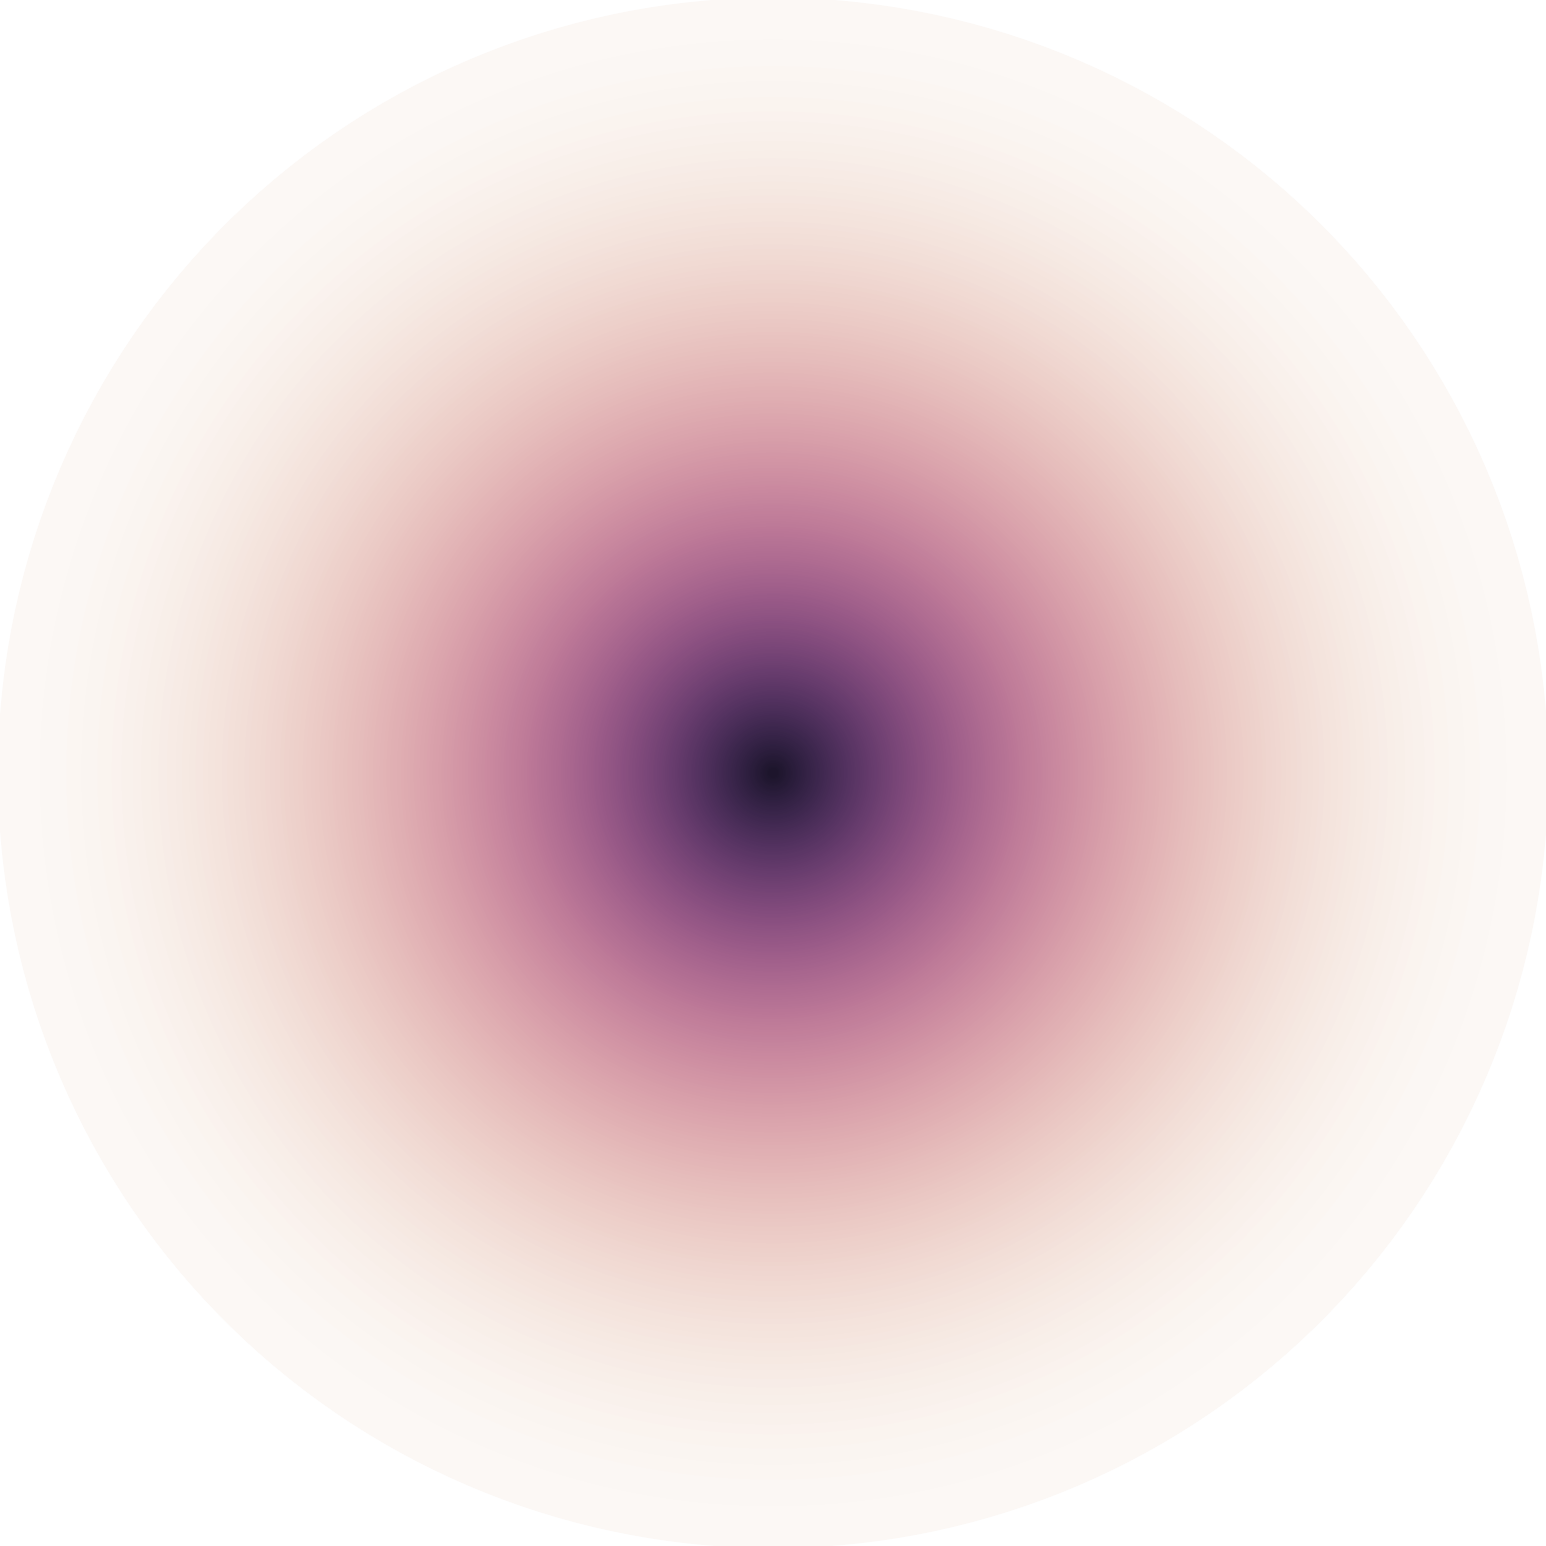
\includegraphics[width=0.35\textwidth]{./img/raw/pl-licht-base.png}};

    \coordinate[] (light-center) at (0,0);
    \node at (light-center) (al) [coord-point, minimum size=\ptsize] {};

    \coordinate[] (lp) at (0.015\textwidth, 0.015\textwidth);
    \node at (lp) (p) [label=above right:{$\mathbf{p}$}] {};

    \draw[black] (light-center) circle [radius=0.175\textwidth];

    \coordinate[] (light-outer) at (0.175\textwidth, 0);
    \draw[-latex] (al) -- (light-outer);

    \coordinate[] (radius-r) at (0.1\textwidth, 0);
    \node at (radius-r) (lr) [label=above:{$\mathit{r}$}] {};
  \end{tikzpicture}
  \caption{Voorstelling van een puntlicht.}
  \label{fig:pl-licht}
\end{figure}

